%%%%%%%%%%%%%%%%%%%%%%%%%%%%%%%%%%%%%%%%%
% Short Sectioned Assignment
% LaTeX Template
% Version 1.0 (5/5/12)
%
% This template has been downloaded from:
% http://www.LaTeXTemplates.com
%
% Original author:
% Frits Wenneker (http://www.howtotex.com)
%
% License:
% CC BY-NC-SA 3.0 (http://creativecommons.org/licenses/by-nc-sa/3.0/)
%
%%%%%%%%%%%%%%%%%%%%%%%%%%%%%%%%%%%%%%%%%

%----------------------------------------------------------------------------------------
%   PACKAGES AND OTHER DOCUMENT CONFIGURATIONS
%----------------------------------------------------------------------------------------

\documentclass[11pt, oneside]{article} % A4 paper and 11pt font size
\usepackage[margin=1in]{geometry}
\geometry{letterpaper}

\usepackage{pslatex}
\usepackage[T1]{fontenc} % Use 8-bit encoding that has 256 glyphs
\usepackage[english]{babel} % English language/hyphenation
\usepackage{amsmath,amsfonts,amsthm} % Math packages

\usepackage{lipsum} % Used for inserting dummy 'Lorem ipsum' text into the template

\usepackage{graphicx} % Required for including pictures
\usepackage{wrapfig}
\usepackage{caption}
\usepackage{subcaption}
\usepackage{float}
\usepackage{enumitem}
\usepackage{listings}
\usepackage{color}
\usepackage[numbers, sort]{natbib}
\usepackage[]{hyperref}


\usepackage{sectsty} % Allows customizing section commands

\numberwithin{equation}{section} % Number equations within sections (i.e. 1.1, 1.2, 2.1, 2.2 instead of 1, 2, 3, 4)
\numberwithin{figure}{section} % Number figures within sections (i.e. 1.1, 1.2, 2.1, 2.2 instead of 1, 2, 3, 4)
\numberwithin{table}{section} % Number tables within sections (i.e. 1.1, 1.2, 2.1, 2.2 instead of 1, 2, 3, 4)

%\setlength\parindent{0pt} % Removes all indentation from paragraphs - comment this line for an assignment with lots of text

\renewcommand{\c}[1]{\texttt{#1}}
\newcommand{\code}[1]{\c{#1}}
\newcommand\todo[1]{\textbf{\textcolor{red}{#1}}}
\newcommand{\teambb}{\c{bennyblum}}
\newcommand{\teamol}{\c{louisofir}}
\DeclareMathOperator{\MD}{MD}
\setlength{\parskip}{1em}

\linespread{1.25}

%----------------------------------------------------------------------------------------
%   TITLE SECTION
%----------------------------------------------------------------------------------------

\title{ 
Tweetnet: Finding the Bots in the Flock\
}

\author{
Josh Blum (joshblum@mit.edu)\\
Bennet Cyphers (bcyphers@mit.edu)\\
Ofir Nachum (ofir@mit.edu)\\
Louis Sobel (sobel@mit.edu)\\
\\
6.857 Final Project
\date{\today}
}

\begin{document}

\maketitle

\vspace{4em}

\begin{abstract}
    Due to Twitter's scale, anonymity, and the reliability of its messaging service, it is an attractive platform to support botnet command and control. The goal of our project was to examine how such a botnet might be implemented and to determine whether such botnets could be detected efficiently. Our approach was to design a game which captures the essential elements of the botnet communication problem. In the game, two teams implement a botnet and each has a limited amount of time to send a random message over a mock Twitter network. The goal is to avoid detection by the other team while discovering the details of the other team's botnet. We ran two rounds of the game under different rules. Based on the results, we conclude that an adversary who takes sufficient design precautions can communicate complex, arbitrary commands over Twitter in a way that is most likely infeasible to detect, even if the source code is compromised.
\end{abstract}

\clearpage

\section {Introduction}
Botnets represent some of the most persistent threats on the internet today. Over the past two decades, the use of networks of hijacked computers for malicious purposes has grown tremendously. A botnet typically consists of a collection of machines infected with a particular malware program which allows the machines to covertly communicate with other infected machines, perform their intended function, and act on commands issued by a central operator. Botnet operators can leverage their armies of ``zombies'' to distribute spam, spread malware, or execute targeted DDoS attacks. Most users of infected computers do not know that they are compromised.

A central aspect of botnet design is the ``command and control'' (C\&C) scheme. The operator must be able to control infected machines in a reliable and scalable manner while avoiding detection and preventing intervention from competing parties. At its core, C\&C requires a way to secretly send messages to thousands of infected machines.

Twitter is an easy-to-use social media platform with a quick signup process, a reliable distributed messaging service, and a robust API. In this project, we looked at the use of Twitter as a platform for botnet C\&C. Our ultimate goal was to detect a botnet ``in the wild''. Along the way, we wanted to determine how such a scheme might be designed, the challenges the designers would face, and what methods could be used for detection. In order to do so, we designed a game where we split our group into two teams, \teambb{} and \teamol{}, and competed to try to communicate a message from a ``master'' to a collection of ``slaves'' on a simplified mock of Twitter. The result is Tweetnet.

\section {Related Work}
Botnets using social networks for C\&C are a relatively recent phenomenon. These botnets take advantage of the reliable infrastructure and easy-to-use APIs of social networks to communicate commands to infected computers. Several of these botnets have already been detected.

Several botnets have been discovered in the wild \cite{arbor, trendmicro, flashback}. In 2009, Arbor Networks \cite{arbor} discovered a Twitter bot which periodically tweets base-64 encoded commands that specify URLs for downloading malicious binaries. The Mehika botnet \cite{trendmicro} is another botnet which was found using Twitter to send commands to its botslaves. The Macintosh Flashback malware provides yet another example of a botnet using Twitter for C\&C \cite{flashback}. The malware queries Twitter for tweets containing specific hashtags.

In addition to these detected botnets, several groups have designed and implemented social networking botnets \cite{socialnetworking, trojan7, stegobot}. A group of San Jose University researchers designed and implemented their \emph{SocialNetworkingBot} to issue commands via Twitter for such things as browsing a URL, taking a screenshot, shutting down the computer, or changing the botmaster \cite{socialnetworking}. Another notable example is \emph{Stegobot}, a botnet which covertly communicates via steganography within images shared on social networks. These examples highlight the ease with which it is possible to use social networks as botnet infrastructure.

In response the the growing threat of botnets using social networks, researchers have proposed several detection mechanisms to thwart such botnets \cite{botsniffer, kartaltepe, burghouwt}. Gu et al. proposed an approach using network-based anomaly detection \cite{botsniffer}. These methods are useful when botnet activity is temporally correlated. Kartaltepe et al. presented a content-specific method which distinguishing natural text from base-64 or otherwise encoded commands \cite{kartaltepe}. The group also suggests client-side detection mechanisms that are alerted by network traffic of dubious origin and purpose.

The previous work in this field shows that while botnets using social networks is a relatively recent phenomenon, the threat of even better concealed botnets is growing rapidly. For this reason, it is imperative that the capabilities of botnet designers be better understood and new detection mechanisms be devised.

\section{Game Overview}
	This section describes the simulation of Twitter we used in order to experiment with bot detection and development techniques.

Twitter processes thousands of tweets per second. Attempting to identify a botnet would be extraordinarily difficult. Instead, we decided to use a mock of Twitter and structure our project as a game.
	
	\subsection{Description}
		We split up the four person group into two teams. Each team would take a turn designing a bot and using it to send information across the mock Twitter infrastructure. The other team would use the resulting stream of tweets to try and determine what the C\&C protocol was and which handle was the botmaster. The defending team would choose what information was transferred and would know the content, timestamps, and username of all tweets.

	\subsection{Justification}
		The use of a game model for security is a reasonable decision. First, it allows simulation of tactics at a small scale. The small scale let us to focus on strategy and cryptography without having to deal with Twitter's massive data stream. Second, there is precedent for such models of security, such as \textsf{IND-CCA}, \textsf{IND-CCP}, and others. In these game models, an adversary is given generous capabilities, such as a ciphertext oracle. If a scheme is secure under these conditions, it can then be considered secure under more relaxed constraints. Our choice of allowing the defending team to choose the information the botmaster needs to transfer was guided by this precedent.

	\subsection{Infrastructure}
		We chose not to play our game actually using Twitter's services, but rather to build a limited subset of them for ourselves. There were three reasons for this. First, we were worried about the ramifications of using automated Twitter accounts on Twitter, including ones that were designed for botnets. Second, some infrastructure would be needed for the game, such as keeping track of when information has been successfully transferred. Since some infrastructure would already be needed, it made sense to create a limited version of Twitter as well. Finally, it made testing and using the bots much more efficient. We didn't have to deal with millions of tweets; we only had to deal with those germane to our game. The infrastructure we built supports basic usernames and tweeting. The code is available on Github\footnote{\url{https://github.com/joshblum/tweetnet}}.

	\subsection{Rules}
		Having given the background on our game, this section now gives a description of the rules.
        
		\begin{itemize}
		 
         \item There are two teams: the attacking team and the defending team. The attacking team is trying to use the mock Twitter as a C\&C channel, while the defending team is trying to catch them.
		 
         \item There is a set number of mock Twitter users. Some handles are \textit{benign} tweeters, which simulate regular people, and the other handles are controlled by the attacking team.
		
         \item The defending team generates random 128 bit hexadecimal \textit{flags}.
		 
         \item The attacking team must pass generated flags to its \textit{bots} using \emph{only} mock Twitter as the communication channel.
		
        \item When a bot receives a flag, it submits it to the defender as proof of successful communication.
        
        \item Bots and botmasters may have arbitrary hard-coded constants for use as shared keys.
        
        \item The botmaster has access to a \textit{random tweet oracle}, which is guaranteed to provide a unique and realistic-looking tweet.
		\end{itemize}

		For enforcement of the rules, we relied on the infrastructure described above and the implicit cooperative understanding between the teams, who would not want to be labelled \textsc{cheaters} in a project.

\section{Round 1}
	This section describes the setup, designs, attacks, and takeaways from the first round of gameplay, for which each team built a botmaster.

	\subsection{Setup}
		During Round 1, each team designed a single \c{Bot} and \c{BotMaster} pair which had to submit a single flag. There were 10 unique handles used. 1 was the botmaster, and the other 9 were benign users, which would tweet with a probability of $0.05$ each second. \teambb{}'s bots knew the botmaster handle at the beginning of the round whereas \teamol{}'s bots established the botmaster as part of their protocol. The goal of this round was to allow the teams to familiarize themselves with the game infrastructure and begin building detection techniques. For this reason, we allowed many simplifications to the game structure for this round, with the intent of modifying the game structure in the subsequent round. 

	\subsection{Designs}
	
		\subsubsection{\teambb{}}
			\teambb{} built the \c{SingleCharBotMaster} which relied on Python's pseudo-random number generator (\c{prng}) to signify tweets which were information carrying. The \c{prng} output stream was used to determine the offset of a single character in each tweet that was information carrying. The botmaster and bots both shared a common seed value for the \c{prng}. Figure~\ref{fig:prng} shows an example of how the \c{prng} was used to offset information tweets, and Figure~\ref{fig:prng-tweet-ex} shows how this offset is used to position a character of the flag within a tweet.

		\begin{figure}[H]
		    \center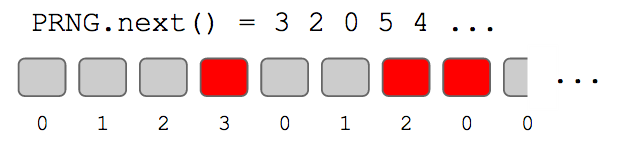
\includegraphics[scale=0.70]{resources/prng.png}
		    \caption{An example of how the \c{SingleCharBotMaster} design uses a \c{prng} to offset which tweets carry information.}
		    \label{fig:prng}
		 \end{figure}

		 \begin{figure}[H]
		    \center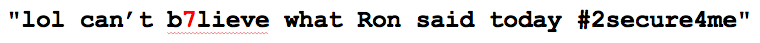
\includegraphics[scale=0.60]{resources/prng-tweet-ex.png}
		    \caption{An example of how the \c{SingleCharBotMaster} design positions flag information in a information carrying tweet.}
		    \label{fig:prng-tweet-ex}
		 \end{figure}
		
			
		\subsubsection{\teamol{}}
			\teamol{} built the \c{SpaceBotMaster}. This botmaster used a space at the end of tweet text to signify a its flag relevance. The master would insert a punctuation mark immediately preceding the space (`.', `,', `!', or `?'), providing two bits of the flag. Two spaces at the end of a tweet signal the start of a flag. Figure~\ref{fig:spacebot} shows an example of a flag-relevant tweet.
            
            \begin{figure}[H]
		    \center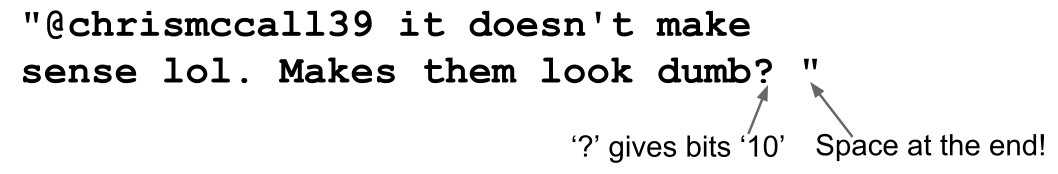
\includegraphics[scale=0.60]{resources/spacebot.png}
		    \caption{An example of how \c{SpaceBotMaster} communicates the flag.}
		    \label{fig:spacebot}
		 \end{figure}

			\teamol{} also put in capabilities for the master to identify itself. The master partitioned time to 12-second windows. When the master tweeted randomly (when it did not have a flag to communicate), it would tweet only in the first 6 seconds of a 12-second window. This way, when the botslaves analyzed user's tweets, they would notice that one had a significant amount of tweets in the first 6 seconds of every 12-second window. They would know this was the master. Unlike the master, any other benign would tweet equally in the first 6 seconds as in the last 6 seconds. In this way, the master is able to discreetly make itself known to the botslaves.

	\subsection{Attacks}

		\subsubsection{\teambb{}}
			The first step in analyzing the data from \teamol{} was to see if there were any inconsistencies from the data set that caused a particular handle to differentiate itself. Using the \c{json} Python module and simple queries across the dataset, the botmaster handle was able to be identified since the frequency of tweeting was twice that of any other handle.

			\teambb{} looked at several techniques in order to identify the master before the handle was found. For example, looking at the frequency of different emoticons and any signal hashtags that may have been used. Once this handle was discovered, \teambb{} wanted to dig deeper into reverse engineering the protocol used.

			Among the set of tweets from the suspect handle, the first thing that stuck out was that many of the tweets had a space character appended to the end of the tweet. This furthered the suspicion that the handle was the botmaster. \teambb{} believed that a binary string was being encoded based on whether the tweet had a space or not.

			Since \teambb{} knew that the botmaster handle was not known to the bots initially, the botmaster would have had to have been established and then the 32 characters of the flag transferred. They tried various transformations of the binary string to convert it to the flag output, without success. 

		\subsubsection{\teamol{}}
	\teamol{} was able to almost entirely discover \teambb{}'s design. They began with visual inspection of the collection of tweets, and immediately noticed aberrations such as \code{r8ally} and \code{RTa@coolman123} -- patterns that did not look anything like what would normally appear on Twitter. \teamol{} further noticed that all of these strange aberrations came from the same username: \c{tweetnet01}.

	Then, they computed tweet frequency by username, and discovered that \code{tweetnet01} had tweeted almost twice as many times as the rest of the usernames had. This cemented their suspicion that \code{tweetnet01} was the botmaster. By visually inspecting all of \code{tweetnet01}'s tweets with a highlighter and pen in hand, \teamol{} was able to find an entire flag embedded in outlying tweets. By examining the pattern of flag character offset and gap between flag tweets, they further identified \teambb{}'s pattern of $n$-down, $n$-over. \teamol{} decided this was based on a \c{prng}, and did not attempt to discover the seed.

	\subsection{Problems}
		From this round we discovered problems both with the game and bot design.
		The game used for this round was an inaccurate representation of Twitter. We allowed many assumptions, such as a very small user base, no social graph interactions, and access to the random tweet oracle. These simplifications gave the attacking teams a great advantage when trying to analyze the bots. For example, any analysis that was done by hand would be unrealistic in the actual Twitter environment without large machine learning or crowd sourcing efforts.
		
		The overarching problem with both bot designs was that the botmasters' tweets prevented them from blending in with the benign tweeters. This showed how difficult steganography can be. Neither team was able to effectively mask the information they wished to hide. These types of errors were coupled with implementation flaws, such as failing to mask the flag content in the \c{SingleCharBotMaster} and misconfiguring the tweeting probability (0.5 was used instead of 0.05).

		We did learn, however, that a high throughput is not necessary for the success of a botmaster. Since many users tweet with a high frequency, even if each tweet from the botmaster relays less than a single bit, not many tweets are needed to communicate with the bots. For example, a botmaster could post a large amount of malicious content (spam) to a public service such as pastebin \cite{pastebin}, and simply use Twitter to communicate the URL to the bots.


\section{Round 2}
	This section is a description of the events of the second round.

	\subsection{Modifications}
		For the second round we introduced several modifications to the game structure. First, the number of bot handles was increased to 20, 2 of which were botmasters. This increased the pool of active handles and gave the designers more flexibility.
		The second major change was that the code of the bots was to be open sourced for the detection team. The bots were allowed a configuration file with predefined constants that could remain remain secret, but all other code was going to be revealed. The motivation behind this was that botnets can be discovered and their source or binary de-obfuscated. The network should be robust to such an attack, and the botmaster handle should be able to remain unknown. 

		
	\subsection{Designs}
		
		\subsubsection{\teambb{}}
        	In the second round, \teambb{} built the \c{HashPadBotMaster}. This bot begins by generating a secret 32-character hex string (the pad) to mask the flag, and a single hexadecimal start signal character. The start character and the pad are generated using an instance of Python's \c{Random} object, which was seeded with a 32-bit secret shared among all bots in the network.
        	
            When the round starts, the botmaster tweets randomly until it receives the flag from the server. Upon receiving the flag, the botmaster sends the start character followed by the 32 characters of the flag XORed with the characters of the pad. Each masked character, $c_i$, is sent in one tweet, chosen at random from a precomputed library of legitimate tweets such that $c_i = \c{hash(tweet)} \pmod{16}$. The botmaster does not send any tweets which hash to the start character until it is ready to send the flag. At all times the master tweets at the same frequency as the legitimate tweeters.
        	
            The listeners consume and discard tweets from the botmaster handle, which they know ahead of time, until one of them hashes to the precomputed start character. At this point, each bot consumes the next 32 tweets, decoding them to characters in the flag according to $f_i = \c{hash(tweet)} \pmod{16} \oplus p_i$, where $f_i$ is the $i^{th}$ character in the flag and $p_i$ is the $i^{th}$ character in the pad. Once all 33 tweets have been consumed, the listener can submit the flag at its leisure, adding jitter to prevent timing correlation attacks.
		
        \subsubsection{\teamol{}}
			\teamol{} built the \c{MD5BotMaster}. When given a flag, one of the two botmaster handles is chosen at random to communicate the flag. This botmaster first masks the flag via a shared \c{prng}. The 32-character masked flag, along with a prepended hexadecimal start signal, is communicated one hex-character at a time in the following way: The bot tweets a tweet with content $c$ such that
			\[
				d=\MD5(\MD5(c)\oplus S_k) \pmod{16},
			\] 
			where $d$ is the desired hex-digit and $S_k$ is a secret key included in the configuration file.

			To further hide the flag communication, the bot does not tweet these flag-relevant tweets in immediate succession. Rather, like the original \c{SingleCharBotMaster}, the botmaster sends between 0 and 4 superfluous tweets between each flag-relevant tweet. The botmaster also tweets a certain number of superfluous tweets before beginning flag communication. Because of the shared \c{prng} seed, the botmaster and the bots
			will stay synchronized.

			To effectively imitate natural communication frequency, \teamol{} implemented a \c{TweetQueue}. Tweets are pushed onto the queue. A single process handles popping and tweeting items from the queue so that a tweet frequency emulating that of the benign tweeters is maintained.
	
    \subsection{Attacks}

		\subsubsection{\teambb{}}

		After reviewing \teamol{}'s code, \teambb{} decided the best attack approach was to try to see which handles, if any, distinguished themselves from the rest. Unlike the previous round, there were no implementation errors that caused obvious deviations. \teambb{} analyzed the mean time between tweets to see if the time to find a tweet with the correct hash was noticeable. 

		\teamol{}'s bots would submit the flag immediately upon decoding it fully. However, since all of the bots tweeted with the same probability, there was no way to distinguish a tweet that occurred close to the flag submission time as originating from the botmaster. 

		\teamol{}'s design was very similar to the design for \teambb{}. However, it did not have the implementation flaws of the \c{HashPadBotMaster} and took advantage of game features such as the random tweet oracle and constant tweet distribution among the benign handles.

		\subsubsection{\teamol{}}
			With \teambb{}'s code in hand, \teamol{} was able to identify the following coding errors and vulnerabilities:  
			
            \begin{enumerate}
				\item To generate a random 128-bit integer, \c{HashPadBotMaster} generates a random float and then multiplies it by $2^{128}$. However, in Python, floats only provide 32 bits of precision, so multiplying $2^{128}$ by a float results in the lower 16 digits as zeros. This means that a significant portion of the flag is communicated unmasked.
                
				\item \c{HashPadBotMaster} uses a single-digit start signal.  This start signal is generated by the faulty random number generator, causing it to always be $0$.
                
				\item \c{HashPadBotMaster} was intended to tweet with a certain probability every second.  This was implemented incorrectly when the bot was not communicating a flag.  At these times, the bot was tweeting with a certain probability every \emph{other} second.
                
				\item \c{HashPadBotMaster} immediately and serially communicates the flag as soon as it obtains it.  Similarly, the botslaves immediately submit it as soon as they decipher it.
                
				\item \c{HashPadBotMaster} does not use a cryptographic hash function but rather Python's built-in \c{hash} function.  This hash function is not pseudorandom and actually very malleable (for example, the hash of ``hello'' is \c{840651671246116861} and the hash of ``helli'' is \c{840651671246116859}).
                
			\end{enumerate}
            
			Due to vulnerability (2), \teamol{} was able to narrow down the search to tweeters which only tweeted a tweet whose hash yields a `0' start signal after the first flag was created.  Subsequently, \teamol{} looked at the 32 tweets following the start signal, and exploited vulnerability (1) to find the partially unmasked flag.  This showed \c{tweetnet16} to be the only candidate botmaster.  This was confirmed via vulnerability (3): \c{tweetnet16} had the lowest number of tweets in the period when there was no flag to be communicated.  \teamol{} was even able to successfully perform a brute-force a search for the randomization seed, which definitively identified \c{tweetnet16} as the botmaster.

			The other vulnerabilities were not used to find the botmaster.  However, given a larger collection of tweets to analyze or more adverse conditions for the detection team, these vulnerabilities could have been exploited to better detect botnet activity.

	\subsection{Problems}
		The main problem that undermined the botnet designs in this round were not protocol issues, but rather coding errors. These are still valid issues to discuss, as actual implementation of a protocol is an important part of applied security. \teambb{} was undermined by an incomplete understanding of the Python numerical model. Errors with under and overflow are a very common source of bugs. Additionally, both teams put too much faith in the default Python \c{prng}. It can easily be brute forced. The number of bits in its seed is only 32 -- even when a Python \code{long} is used as the seed, Python internally uses the \c{hash} value of that long, which is only 32 bits. These issues are implementation issues, not protocol ones. Mistakes like these are a common source of security issues, and it is possible that Python is not a suitable language for designing cryptographic protocols.

\section{Discussion}
	This section presents a discussion of the results above. We discuss what we learned, the applicability of our project to the actual Twitter service, and possible future work.

	\subsection{What we learned}
		Through our iterative game, we realized the challenges faced by botnet design and detection teams. First, we realize that tweet frequency is a key aspect of any botnet and can often be a botnet's most vulnerable component. In the first round of gameplay, both teams were unsuccessful at achieving a natural tweet frequency. This single flaw was clearly visible to botnet detection teams and made identifying the botmaster easy. In the second round, even with the lessons of the first round learned, \teambb{} still made mistakes which led to detectable and unnatural tweet frequencies. This shows that making frequency of communication natural is a key goal for designers of botnets using social networks. Although this is a feasible goal, it is very easy to get wrong. From the botnet detection perspective, characterizations of natural communication frequency and tools to detect deviations from this frequency would be quite useful.

		Another key aspect is natural tweet content. In Round 1, both teams used communication methods that altered tweet text. These methods were easily detected. This shows that even seemingly concealing communication tactics that change natural text (like single character alterations) are not enough to hide information. However, botnet designers can thwart this by using the hashing method used by both teams in Round 2. Despite this work around, it is still very important for detection teams to have a tool for distinguishing natural from unnatural text, as many botnet designers may overlook this vulnerability.

	\subsection{How this extends to real Twitter}
	Some of what we've learned about detecting and creating C\&C channels over our mock Twitter can be applied to the actual Twitter service. One thing is the ease of hiding information in a tweet by using the hash of a randomly generated and realistic looking tweet. This technique could definitely be used to send significant amounts of information covertly. Another thing we learned that does extend to real Twitter is that for a botnet to be successful, it would not need to transfer large amounts of data over the C\&C channel. Information on the order of bytes is sufficient to serve as a pointer to further instructions for the botnet. Twitter may be just one component of an elaborate C\&C scheme.

	\subsection{How this does \textit{not} extend to real Twitter}
    A related problem is that of spambots. Spambots are computer-controlled Twitter handles which tweet out ads, links, and otherwise annoying messages on behalf of a company or anonymous mischief-maker. Spam detection is difficult. Several papers have been written on techniques for identifying these bots among the large datasets that Twitter produces \cite{botdetect, spambotML, socialnet_spam}. As detection techniques advance, spambots evolve to compensate. Furthermore, since the goal of spambots is to send information for human consumption, they are restricted to messages in plain text or URLs. Botnets using Twitter are not hampered by such limitations. As  we have demonstrated, information can be carried by sequences of arbitrary  tweets using hashing, so a botmaster only needs a sufficiently sized  library of legitimate-sounding tweets to be able to transmit any possible message. Therefore, it seems likely that any botnet with sufficiently motivated operators can evade automated bot detection comparatively easily.
 
In our tests, there were a small number of handles providing background noise in a very predictable fashion. This made it easy to look for subtle variations in timing and content in each handle's tweets and to perform extensive analysis on each one. The real Twitter stream consists of millions of handles with wildly varying tweet patterns in several languages, so it is much more difficult to identify breaks from general trends. For example, \teambb{}'s botmaster in Round 2 was identified in part because it tweeted half as frequently as normal handles. In reality, the normal range of tweet frequency spans orders of magnitude (anywhere from several times an hour to once or twice a year), so it would be unrealistic to use this metric alone to identify bots. In addition, it is computationally infeasible to analyze any significant fraction of Twitter's entire tweet stream at the level of detail that we were able to.
        
        \subsection{Future Designs / work}

        The current mock Twitter infrastructure could be extended to modify the gameplay and make the simulation more realistic. Some aspects of gameplay were never explored, such as analyzing the social graph through followers or having a distribution of benign user behavior. Modifying these parts of the infrastructure would change how the detecting teams could perform their analysis and move the detection closer to what it would be like when using real tweets.

		Another feature that could be modified is the botmaster's access to a random tweet oracle. This assumption allowed the botmaster to generate realistic tweets on demand, an ability which is quite complicated in real life. Forcing botmasters to develop their own tweets (or only retweet those of other users) would make the job of the botmaster much more difficult. It would be a realistic challenge that a botnet would face if they wished to hide their C\&C channel within Twitter.

\section{Conclusion}
     	Botnets are hard to build. In any implementation, there is a good chance that subtle errors in design will lead to identifiable patterns in the output. However, if enough security precautions are taken, we believe it is possible to design a cryptographically secure scheme that is very difficult to detect. The volume and variety of data in Twitter's stream are also obstacles to detection. Any detection mechanism deployed on Twitter will have to be efficient and scalable. Some of the methods we used were not. Regardless, we produced a good framework for modeling the use of Twitter for the command and control of botnets.

        

\clearpage
\renewcommand\bibsection{\section{References}}
\renewcommand*{\bibfont}{\footnotesize}
\setlength\bibsep{3pt}
\bibliographystyle{ieeetr}
\bibliography{tweetnet}

\end{document}
